% fig-race.tex: two devices storing from the same version, with the upload first and with the head first (draft of 6 Nov 2026).
% Build from this folder:  pdflatex fig-race.tex     The blue arrows are requests about the head, as in the other figures.
% Source: section 4.4, the paragraph "Reserve first", and the first rejected alternative of section 4.6.
% Not run: this interleaving is the reasoning of the design (Table 6.5 says which two-device cases were run).
\documentclass[tikz,border=4pt,11pt]{standalone}
% style.tex: what the four diagrams share (colours, fonts, the look of a party, a message, a note).
% The one accent colour is the blue of the latency charts; it always means "the head", the thing this thesis adds.
% Everything else is black or grey, so the figures still read when printed in black and white.
\usepackage[T1]{fontenc}
\usepackage{mathptmx}
\usetikzlibrary{positioning,calc,arrows,fit,backgrounds}
\definecolor{head}{HTML}{2A78D6}
\definecolor{ink}{HTML}{0B0B0B}
\definecolor{inktwo}{HTML}{52514E}
\definecolor{soft}{HTML}{F0EFEC}
\definecolor{rule}{HTML}{C3C2B7}
\tikzset{
  every picture/.style={font=\small, >=latex},
  party/.style={draw=ink, fill=soft, rounded corners=2pt, minimum width=3.4cm, minimum height=0.8cm, align=center, font=\small\bfseries},
  box/.style={draw=ink, fill=soft, rounded corners=2pt, minimum width=3.9cm, minimum height=1.9cm, align=center},
  quiet/.style={draw=rule, text=inktwo},
  life/.style={draw=rule, line width=0.9pt},
  msg/.style={->, draw=ink, line width=0.7pt},
  rep/.style={->, draw=ink, line width=0.7pt, dashed},
  hmsg/.style={->, draw=head, line width=1.2pt},
  hrep/.style={->, draw=head, line width=1.2pt, dashed},
  bad/.style={->, draw=ink, line width=1.2pt, dashed},
  lab/.style={font=\footnotesize, inner sep=3pt, text=ink},
  act/.style={font=\footnotesize, align=left, text=ink, fill=white, draw=rule, rounded corners=1.5pt, inner sep=3pt},
  outcome/.style={font=\footnotesize, align=center, text=ink, fill=white, draw=ink, rounded corners=1.5pt, inner sep=4pt},
  side/.style={font=\footnotesize\itshape, align=left, text=inktwo},
  band/.style={fill=soft, draw=rule, rounded corners=2pt, minimum height=0.7cm, font=\footnotesize, text=inktwo},
  holds/.style={font=\footnotesize, text=inktwo, fill=white, draw=rule, rounded corners=1.5pt, inner sep=2.5pt},
}

\tikzset{
  party/.append style={minimum width=2.9cm},
  lab/.append style={fill=white, inner sep=1.5pt},
}
\begin{document}
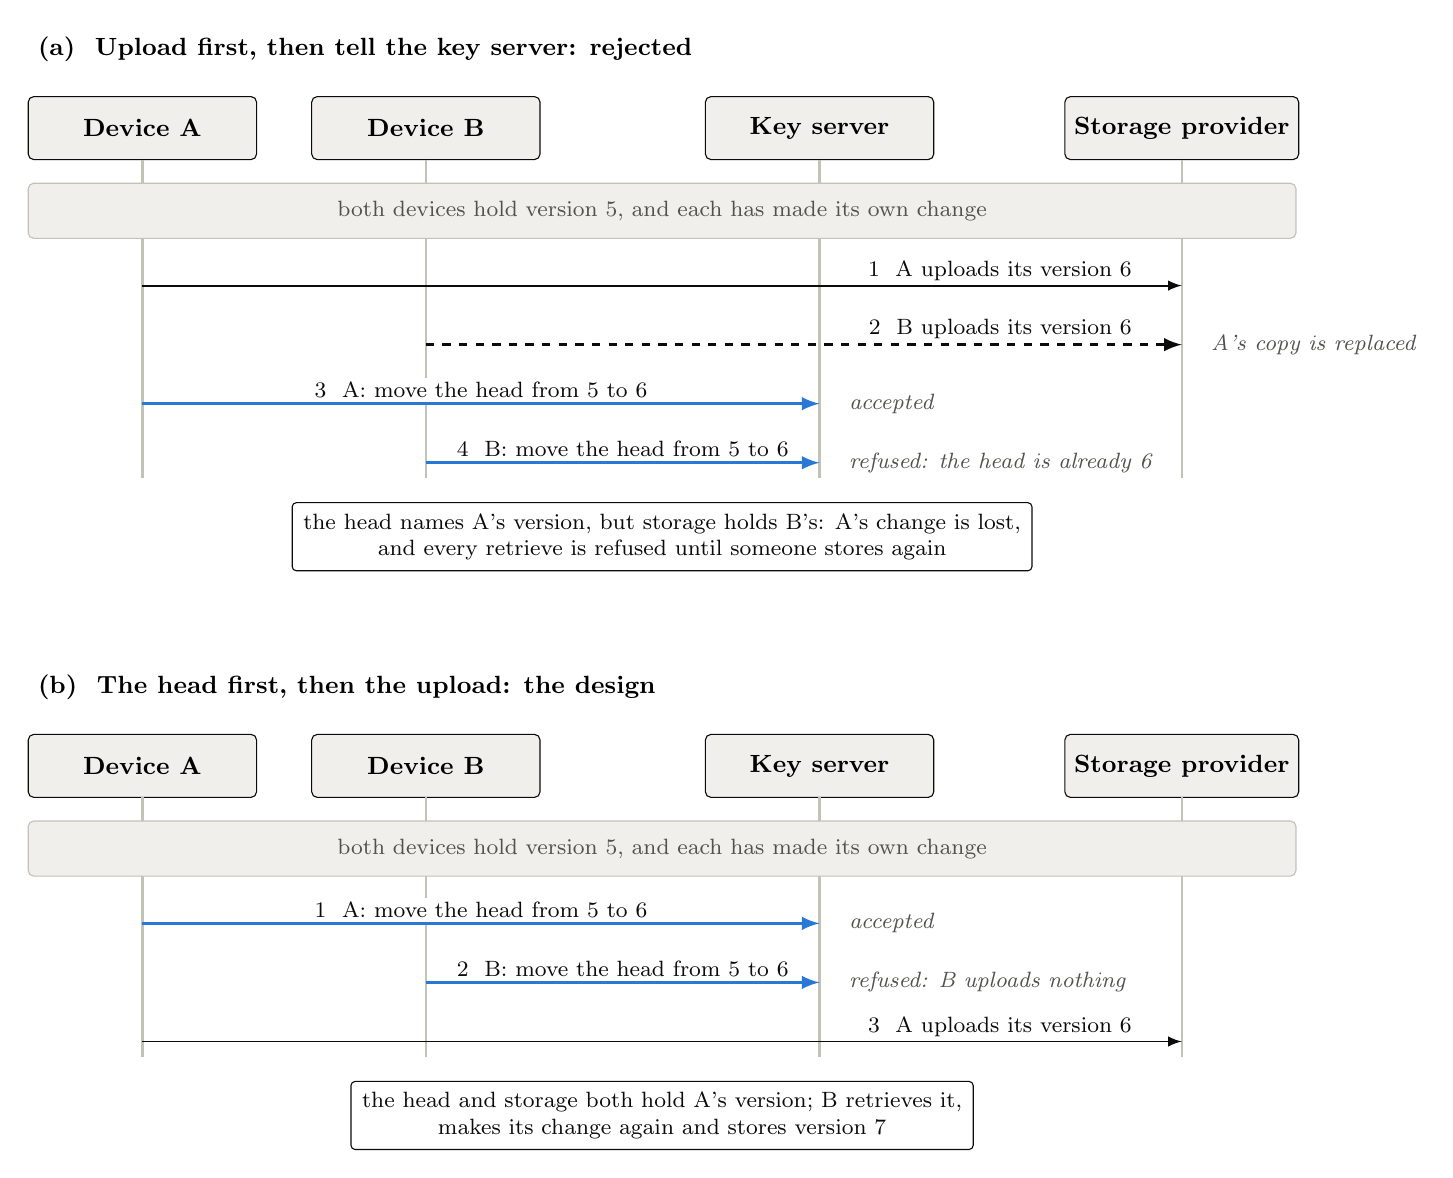
\begin{tikzpicture}
% ---------------------------------------------------------------- (a) upload first
\node[font=\small\bfseries, anchor=west] at (-1.45,1.0) {(a)\ \ Upload first, then tell the key server: rejected};
\node[party] (A) at (0,0)    {Device A};
\node[party] (B) at (3.6,0)  {Device B};
\node[party] (K) at (8.6,0)  {Key server};
\node[party] (D) at (13.2,0) {Storage provider};
\foreach \x in {0,3.6,8.6,13.2} \draw[life] (\x,-0.4) -- (\x,-4.45);
\node[band, minimum width=16.1cm] at (6.6,-1.05) {both devices hold version 5, and each has made its own change};
\draw[msg]  (0,-2.0)   -- node[lab, above, pos=0.825] {1\ \ A uploads its version 6} (13.2,-2.0);
\draw[bad]  (3.6,-2.75) -- node[lab, above, pos=0.76] {2\ \ B uploads its version 6} (13.2,-2.75);
\node[side, anchor=west] at (13.45,-2.75) {A's copy is replaced};
\draw[hmsg] (0,-3.5)   -- node[lab, above, pos=0.5] {3\ \ A: move the head from 5 to 6} (8.6,-3.5);
\node[side, anchor=west] at (8.85,-3.5) {accepted};
\draw[hmsg] (3.6,-4.25) -- node[lab, above] {4\ \ B: move the head from 5 to 6} (8.6,-4.25);
\node[side, anchor=west] at (8.85,-4.25) {refused: the head is already 6};
\node[outcome, anchor=north] at (6.6,-4.75) {the head names A's version, but storage holds B's: A's change is lost,\\ and every retrieve is refused until someone stores again};
% ---------------------------------------------------------------- (b) reserve first
\begin{scope}[yshift=-8.1cm]
\node[font=\small\bfseries, anchor=west] at (-1.45,1.0) {(b)\ \ The head first, then the upload: the design};
\node[party] (A2) at (0,0)    {Device A};
\node[party] (B2) at (3.6,0)  {Device B};
\node[party] (K2) at (8.6,0)  {Key server};
\node[party] (D2) at (13.2,0) {Storage provider};
\foreach \x in {0,3.6,8.6,13.2} \draw[life] (\x,-0.4) -- (\x,-3.7);
\node[band, minimum width=16.1cm] at (6.6,-1.05) {both devices hold version 5, and each has made its own change};
\draw[hmsg] (0,-2.0)   -- node[lab, above, pos=0.5] {1\ \ A: move the head from 5 to 6} (8.6,-2.0);
\node[side, anchor=west] at (8.85,-2.0) {accepted};
\draw[hmsg] (3.6,-2.75) -- node[lab, above] {2\ \ B: move the head from 5 to 6} (8.6,-2.75);
\node[side, anchor=west] at (8.85,-2.75) {refused: B uploads nothing};
\draw[msg]  (0,-3.5)   -- node[lab, above, pos=0.825] {3\ \ A uploads its version 6} (13.2,-3.5);
\node[outcome, anchor=north] at (6.6,-4.0) {the head and storage both hold A's version; B retrieves it,\\ makes its change again and stores version 7};
\end{scope}
\end{tikzpicture}
\end{document}
